\documentclass{article}
\usepackage[utf8]{inputenc}

\usepackage{booktabs}
\usepackage{tabularx}
\usepackage{graphicx}
\usepackage{xcolor}
\title{SE 3XA3: Development Plan}

\author{Team 10, MacLunky
		\\ Albert Zhou, zhouj103
		\\Abeer Al-Yasiri, alyasira
		\\ Niyatha Rangarajan, rangaran
}


\date{April 12, 2021}


\begin{document}


\begin{table}[hp]
\caption{Revision History} \label{TblRevisionHistory}
\begin{tabularx}{\textwidth}{llX}
\toprule
\textbf{Date} & \textbf{Developer(s)} & \textbf{Change}\\
\midrule
February 4, 2021 & Albert, Abeer, Niyatha & Version 0 made\\
\hline
\textcolor{red}{April 11, 2021} & \textcolor{red}{Abeer} & \textcolor{red}{POC plan, Poject Review}\\
\bottomrule
\end{tabularx}
\end{table}


\newpage

\maketitle

This document will explore the development plan of MacLunky project in terms of team logistics, project design, testing plan, and project execution.

\section{Team Meeting Plan}

Meetings will occur at the following times: Tuesday 2:30pm to 4:30pm and Thursday 7:00pm to 9:00pm on MS Teams. Additional meetings will be scheduled at the team's discretion. A different member will direct the meeting agenda week. It includes: discussion of individual progress, peer review of completed work, expectations for next meeting, group decisions, discussion with TAs, conflict resolution, git committing. Meetings will be recorded by Albert.

\section{Team Communication Plan}

\begin{enumerate}
    \item The development team will use GitLab to track the development progress of the project and to share all code and files. Also, the team will use the "To Do List" and "Issue" features on GitLab to comment on the development files and keep the team up to speed on the project's progress.
    \item The development team will use Microsoft Teams as means for team meetings. 
    \item The development team will use Facebook Groups for direct and fast line of communications and to share announcement and ask project related questions.
\end{enumerate}

\section{Team Member Roles}
The development team has decided to take a different approach on selecting a team leader and it entails for every project milestone a member will be assigned as the leader. Hence, every member will have the opportunity to showcase their leadership skills. 
The scribe of the team will be Albert. Albert is responsible for the meeting documents and setting up the milestones documents. Niyatha will be responsible for submitting documents through GitLab and maintaining the team's Git repo updated. Also, Niyatha will be the team's expert on LaTex related issues and managing the development documentation. Abeer will be responsible for researching and providing information for the project development's technology. This includes downloading and implementing the required tools for testing and project implementation. 

\begin{table}[h!]
    \centering
    \begin{tabular}{|c|c|}
         \hline
         Name & Role\\
         \hline
         Abeer & Milestone (1,4,7,10) leader, Technology.\\
         \hline
         Albert & Milestone (2,5,8,12) leader, Scribe.\\
         \hline
         Niyatha & Milestone (3,6,9) leader, GitLab, Latex, Documentation \\
         \hline
    \end{tabular}
    \caption{Team Roles}
    \label{tab:my_roles}
\end{table}

\section{Git Workflow Plan}
%Feauture Branch workflow plan??

The team will use a centralized git strategy. The main branch will contain all final versions of source code and documents. This will allow the team to work concurrently on the same files. Also, this prevents any issues stemming from merging branches. Members will communicate issues directly through MS Teams/Facebook or by using git issues. Labels will be used for identifying bugs, notifying merge request, new documents, new features, and marking old versions. Milestones will be used to track the dates of deliverables and features based on the Gantt Chart.

\section{Proof of Concept Demonstration Plan}

The proof of concept demonstration will include showing the overall design architecture of the project and the user interface of the system. The plan is to use Python 3 and Pygame to demonstrate the system's functionality and prove the project's feasibility. Also, part of the plan is to describe the scope of the project; that is to redesign the graphical feature of the system and introduce more gaming functionalities. \\
Moreover, the architecture design will be presented in the form of a summary of the system's functional features and the breakdown of the development modules of the project. The team plan to use the Model-View-Controller pattern \textcolor{red}{in a custom format} to guide the development of the modules. Modules relating to the game can be combined to form the model. Views can show or hide details of the game to each type of user like players, testers, and developers. A controller can easily connect the user's inputs to changes in the model. \textcolor{red}{The customized pattern the team decided to adopted included a main file that acts as the controller for connecting the different game modules and as the view to display the game by using the view module through method calls.} Additionally, the proof of concept demonstration will present a dashboard UI to illustrate the different functionalities of the project module's and the user experience with the system.\\
Furthermore, the proof of concept will focus on discussing the challenges and advantages of using Python 3 and Pygame in the implementation process from the developer's point of view. A very important project risk is scalability of the software to meet the project's scope. This includes problems with module design related to performance, maintainability and security aspects of the game. For example, failing to ensure proper separation of concerns in the design could lead to maintainability issues and difficult testing plans. This can be shown by using Unit testing for small modules to be simple and somewhat automated. Testing multiple modules together would be difficult as it cannot be automated. Also, the risk upon expanding the original Pylunky project may be difficult since the project was not meant to include many modules. It was just a simple framework for the game functionality. Hence the plan must highlight how the new modules fit well with the original ones. The team will have to either adapt the new modules or change the existing ones. Another important project risk is the re-implementation of the original Python 2 game to Python 3 that might not include all the features of the original game. Such problems could come from the difference of how Pygame interacts with the different Python versions. Therefore, the proof of concept must provide an exactly re-implementation of the previous game and point out if additional technology was required and showcase one new game feature to verify the advantage of using Python 3. Pygame can not be used to create high resolution 3d images and has a tendency to not be responsive in certain terminals. However, it can still be used to create high level games with reasonable performance and hence, we choose to use it regardless of these limitations. Therefore, the proof of concept plan must deliver a demonstration of how to mitigate for such risks.\\
Also, the demonstration will explain what design decisions must be taken to ensure that the system will be easy to install for the user. Not only that, the proof of concept will outline the testing plan of the project and what testing technique will be used and for what purpose. A tester must carefully set up the state of the system, observe the correct behaviour of modules, and verify that all of their interactions with each other are correct. With many modules, testing could be very resource intensive, leading to wasting resources for little payoff or incomplete testing results\\
Additionally the project's portability should not be a concern as the system runs on the Python Virtual Machine, so any machine with Python should be able to use the system.\\
In general, the proof of concept demonstration will show the project's design decisions, design risks, and technical feasibility.

\section{Technology}
\subsection{Programming language}
The programming language our project is centered around is Python3. Python3 particularly offers multiple libraries that would help in game development. The team have chosen to work with Pygame. The original version of this project made use of Python2 and Pygame. However, there were sources of potential errors in the initial code. Keeping this in mind we plan to integrate the game into a more current version - Python3. The initial version had only a small scale prototype with limited functionalities. Using Pygame the team plans to widen the scope of the game by adding more sophisticated functionalities.
\subsection{IDE and Testing Framework}
In terms of the IDE or coding environment we plan to use VS code. This environment is most suitable for achieving a number of project development stages namely testing, documentation and coding. VS code offers compatible plug in environments based on the code written in a file. It also offers lint, git, etc. addons which will be useful during the testing stages. PyLint helps maintain clean and readable code. It is most useful in a team environment and hence using it through VS code is most optimal. Furthermore, pytesting and unit testing environments are built in and thus, it increases efficiency of code performance by mainly using one platform. 
\subsection{Documentation}
Documenting code is one of the most important steps in a group environment especially when one teammate wishes to communicate their ideas efficiently. Using the Ubuntu environment, one can easily download relevant packages concerning Doxygen and Latex. Together with VS code's terminal one can easily run code, compile it with a python environment and finally create automatic documentation using Doxygen templates.\\\\
Using the Git addons feature of this platform we will be frequently committing our code to our team git repo to maintain and provide a centralized access to the said code.


\section{Coding Style}
%https://code.visualstudio.com/docs/python/linting#_pylint
Since the project's coding structure follows Python3 we will be using the default linting standards set by VS code for Python. This follows the Pylint rules. Pylint is able to catch a number of bugs and even allows certain 'known bugs' to pass and disable unimportant warnings. Furthermore, functions in the program will take default values if they are not provided.

\section{Project Schedule}
The Gantt chart can be found in the Project Schedule folder of the GitLab repository. The images of the said chart are below as well:
\begin{center}
    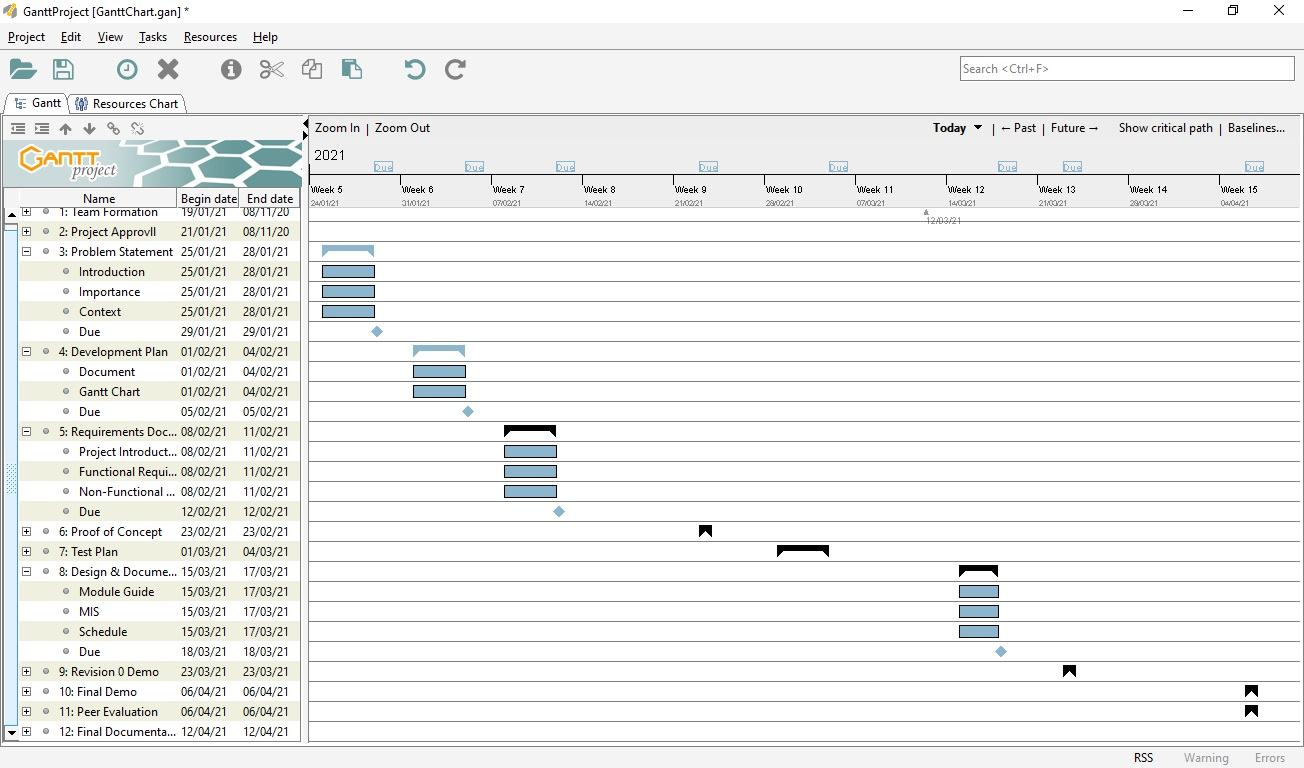
\includegraphics[scale=0.4]{Gantt1.jpg}
    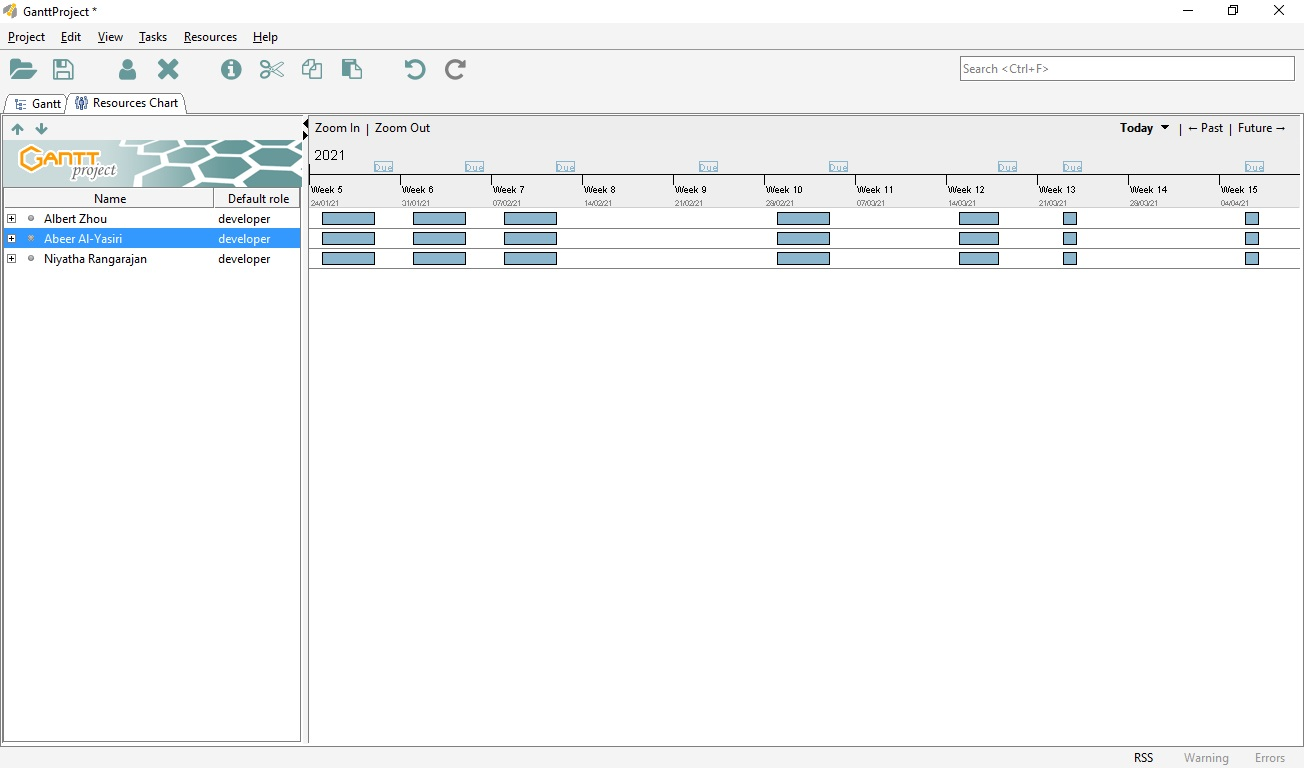
\includegraphics[scale=0.4]{Gantt2.jpg}
\end{center}

\section{Project Review}
\textcolor{red}{Considering the time constraints and the project's scope, the execution of the project plan went very well. The team was able to meet all the course deadline for the documents and the development deadlines that was set by the development team. The team communicated effectively with each other and provide continuous support during the development process by adapting a peer programming style to edit and track the progress of the code. Not only that the project was thoroughly analyzed from the design pattern perspective to produce a modular and well documented code that could be easily maintained and added to in the future. The project was very successful in meeting and fully implementing the functional requirements of the project and in producing a user friendly product. This shows that the project followed the preset development plan very well and was able to present a system that be of interest to the target audience. Not only that the team provided an exhaustive reports and documentation of the development plan that reinforces the quality of the produce.\\
However, even though the project was successful in meeting the main goals of the project some areas code have been better explored during the development plan that would have allowed for more aggressive testing techniques to be applied on the system during the testing phase. Therefore, in the future the development plan should include more details on the various technology available to the project and what is the potentiality of the technology actually being useful further down the development process. By doing early on research of the available technology then the team could allocate more time with exploring only the useful technology and hence exploring more areas in the project that might have been neglected during this run such as performance issues, coverage testing, and look and feel user feedback. Overall, the project was a success because the team delivered a functional system that meets the scope and in future versions of the system the team could explore and enhance user experience further given the more time.}

\end{document}
